\documentclass[a4paper,11pt]{article}
\usepackage[margin=20mm]{geometry}
\usepackage[T1]{fontenc}
\usepackage[utf8]{inputenc}
\usepackage{lmodern,amsmath,amssymb,booktabs,longtable,graphicx}
\usepackage[round]{natbib}
\usepackage[hidelinks]{hyperref}
\usepackage{microtype,tikz}
\usetikzlibrary{arrows.meta,positioning,calc}
\setlength{\emergencystretch}{3em}
\setlength{\tabcolsep}{4pt}
\title{RC-QASyn: Auditable Evidence, Coverage-Aware Construction and Bounded Repair for Synthetic Tabular Data}
\author{Author names and affiliations to be supplied by the research team}
\date{Empirical revision --- 25 October 2026}
\begin{document}
\maketitle
\begin{abstract}
Among 601 historical synthetic tabular candidate occurrences from three imbalanced classification datasets, 75 (12.5\%) violate source-declared structural requirements; page-blocks0 accounts for 64 violations among 200 candidates (32\%). RC-QASyn makes these defects, statistical support and dataset contribution separately auditable through provenance, schema checks, local and global TRAIN evidence, descriptive admission, fixed-budget construction and bounded integer repair. All 54 eligible repairs become structurally compliant; 21 rejected records remain ineligible. At matched budgets, quality-coverage selection raises distinct-feature TRAIN coverage over source order from 0.622 to 0.948 on Abalone19 and from 0.416 to 0.506 on Ecoli4, with zero exact duplicates. Improved geometry does not ensure improved classification: expanding the repaired page-blocks0 pool lowers logistic pure-synthetic F1 from 0.446 to 0.342 (paired conditional 95\% difference interval: $[-0.135,-0.074]$). A separate train-only offline study uses five fresh stratified splits per dataset. Curated augmentation yields mean F1 $0.758\pm0.166$ on Ecoli4 versus $0.848\pm0.119$ for real-only training; gains on page-blocks0 are small and random curation remains competitive. Saved predictions support 2,000-resample paired intervals. These results establish reproducible structural and geometric effects with mixed utility outcomes, without independently establishing complete semantic validity.
\end{abstract}
\noindent\textbf{Keywords:} synthetic tabular data; curation; coverage; bounded repair; imbalanced learning.

\section{Introduction}
A generated record can be readable and numerically plausible while omitting its class, violating an integer declaration or duplicating another record. These failures occur in the studied population: 75 of 601 candidates violate authoritative structure, including 64 of 200 page-blocks0 records. These are rates for this historical generation campaign, not estimates for LLM outputs generally. They motivate checking what a record contains before interpreting distributional resemblance or downstream usefulness.

Three questions remain distinct. Does a candidate comply with justified source declarations? How well does it resemble TRAIN observations locally and globally? What does it contribute to a selected dataset and its classifier? A distant observation may be legitimate, a compliant record may be redundant, and a diverse subset may train a worse classifier. RC-QASyn addresses these distinctions with an auditable curation system.

We ask: to what extent do structural filtering, heterogeneous evidence, coverage-aware selection and bounded repair improve measurable synthetic-data characteristics and downstream classification utility compared with simple alternatives? The revision combines a controlled historical study with a separate offline replication. Annotation experiments and validity calibrators are outside the active scope.

The contributions are:
\begin{enumerate}
\item Auditable separation of source-schema compliance, local/global statistical support and dataset contribution, linked to immutable candidate identities.
\item Evidence-aware fixed-budget construction evaluated against random, source-order, farthest-first and coverage-greedy controls, with coverage and redundancy measurements.
\item Source-preserving bounded integer repair, controlled reevaluation and matched-budget measurement of structural, geometric and utility changes.
\item Empirical analysis of agreement and disagreement between geometry and classification, strengthened by paired prediction uncertainty and split-specific offline generation.
\end{enumerate}
These are integration and empirical contributions. Distances, covariance regularization, greedy selection, oversampling and bootstrap methods are established components; no new optimality guarantee is claimed.

\section{Related work}
CTGAN, TabDDPM and GReaT model tabular generation through conditional adversarial, diffusion and language-model approaches \citep{xu2019ctgan,kotelnikov2023tabddpm,borisov2023great}. RC-QASyn curates an existing candidate stream. The historical generator is not retrained here, and offline experiments do not reproduce its LLM behavior.

Synthetic-data evaluation can distinguish fidelity, diversity and generalization \citep{alaa2022faithful}. Our TRAIN coverage and duplication rates are narrower diagnostics, without that work's probabilistic or privacy interpretation. Constraint-aware models incorporate explicit constraints into generation \citep{stoian2024realistic}. RC-QASyn checks justified declarations after generation and permits a narrower integer-only correction.

Greedy coverage and diversity-based subset selection have substantial prior literature \citep{nemhauser1978submodular,sener2018coreset}. We reuse these ideas with traceable admission, class quotas and duplicate suppression. Classical unconstrained greedy guarantees do not automatically extend to the combined lexicographic selector.

SMOTE interpolates minority observations \citep{chawla2002smote}. We use established imbalanced-learn implementations, including mixed-type SMOTENC \citep{lemaitre2017imbalanced}. Oversampling is a generation/training baseline, random candidate selection is a curation control, and class weighting changes classifier training. They answer different questions.

Calibration concerns agreement between confidence and observed outcomes \citep{guo2017calibration}; candidate percentiles lack that interpretation. Bootstrap inference depends on its resampling design \citep{efron1979bootstrap}, and supplementary Wilson recall intervals address small positive counts \citep{brown2001interval}. Synthetic-data surveys and LLM-judge studies motivate traceability while limiting what recorded critic decisions establish \citep{long2024survey,zheng2023judging}.

\section{Methodology}
Let $T$ denote REAL TRAIN, $E$ REAL TEST and $G=\{(o_i,x_i,y_i)\}$ the candidate stream. Occurrence identity distinguishes physical records even when payloads are equal. Source files, ordinals, payload hashes, specifications and experiment identities link each selected record to its inputs. Missing class remains missing; generation conditioning never supplies an absent payload label.

\begin{figure}[p]\centering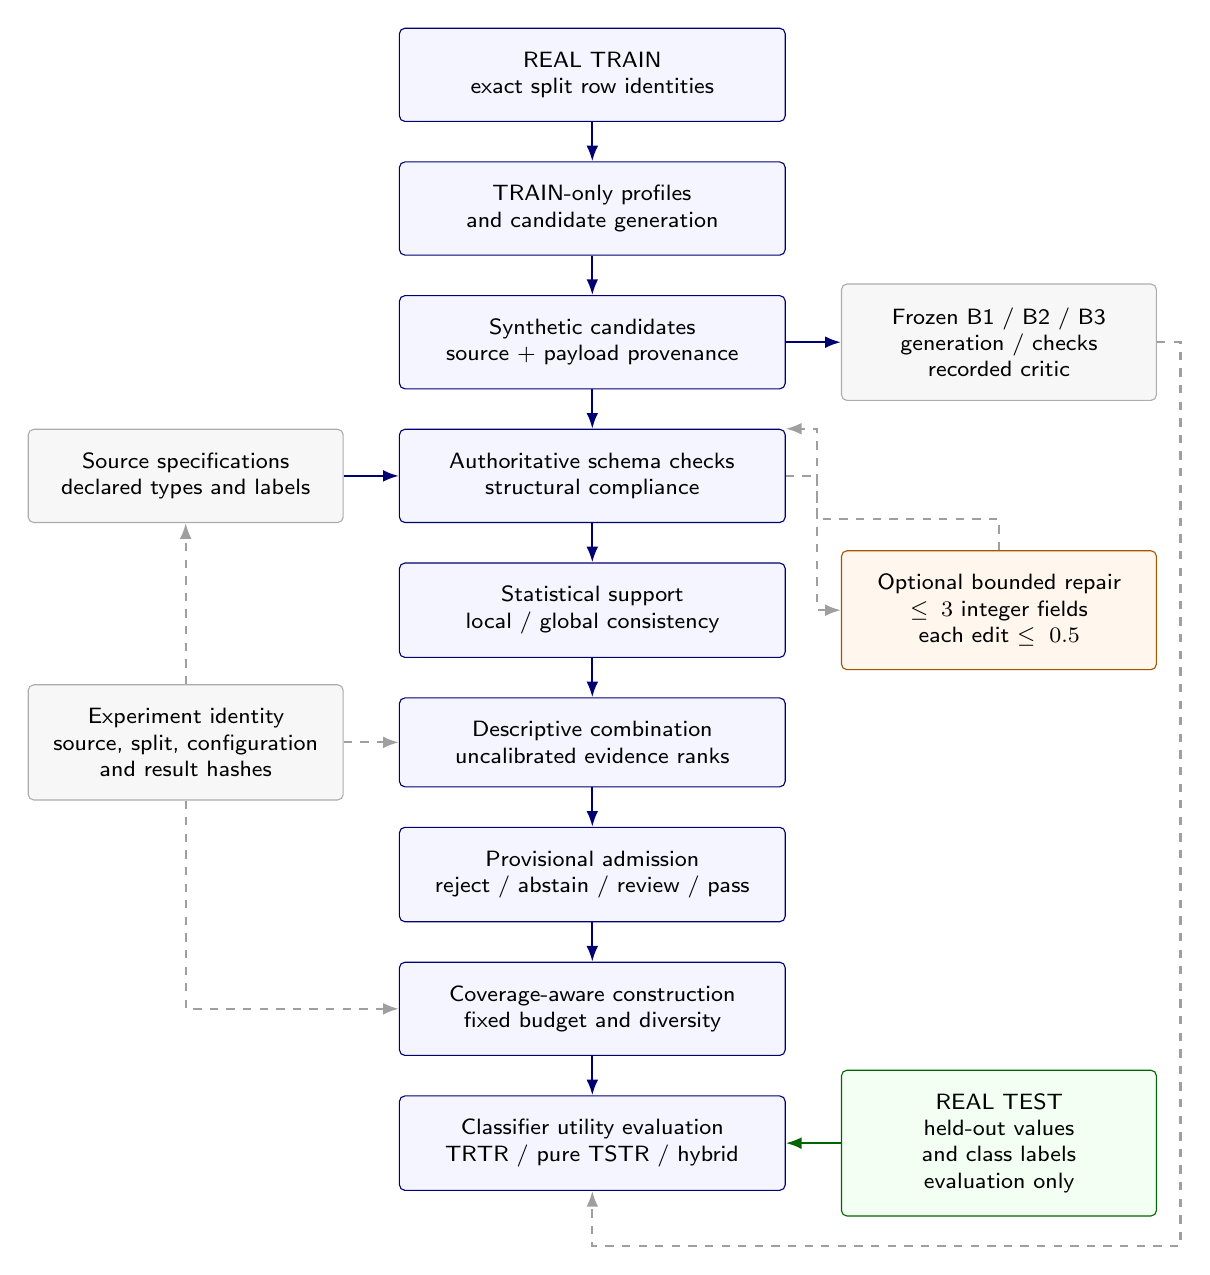
\begin{tikzpicture}[font=\sffamily\footnotesize,
 box/.style={draw=blue!45!black,fill=blue!4,rounded corners=2pt,align=center,text width=43mm,minimum height=10mm,inner sep=3mm},
 side/.style={box,text width=34mm,fill=gray!6,draw=gray!65},
 flow/.style={-{Latex[length=2mm]},thick,draw=blue!45!black},
 audit/.style={flow,dashed,draw=gray!75},node distance=5mm]
\node[box] (train) {REAL TRAIN\\exact split row identities};
\node[box,below=of train] (fit) {TRAIN-only profiles\\and candidate generation};
\node[box,below=of fit] (candidate) {Synthetic candidates\\source + payload provenance};
\node[box,below=of candidate] (schema) {Authoritative schema checks\\structural compliance};
\node[box,below=of schema] (evidence) {Statistical support\\local / global consistency};
\node[box,below=of evidence] (fusion) {Descriptive combination\\uncalibrated evidence ranks};
\node[box,below=of fusion] (admit) {Provisional admission\\reject / abstain / review / pass};
\node[box,below=of admit] (select) {Coverage-aware construction\\fixed budget and diversity};
\node[box,below=of select] (eval) {Classifier utility evaluation\\TRTR / pure TSTR / hybrid};
\node[side,left=7mm of schema] (spec) {Source specifications\\declared types and labels};
\node[side,left=7mm of fusion] (identity) {Experiment identity\\source, split, configuration\\and result hashes};
\node[side,right=7mm of candidate] (controls) {Frozen B1 / B2 / B3\\generation / checks\\recorded critic};
\node[side,right=7mm of evidence,fill=orange!7,draw=orange!65!black] (repair) {Optional bounded repair\\$\le3$ integer fields\\each edit $\le0.5$};
\node[side,right=7mm of eval,fill=green!5,draw=green!40!black] (test) {REAL TEST\\held-out values\\and class labels\\evaluation only};
\foreach \a/\b in {train/fit,fit/candidate,candidate/schema,schema/evidence,evidence/fusion,fusion/admit,admit/select,select/eval}
 \draw[flow] (\a) -- (\b);
\draw[flow] (spec) -- (schema);
\draw[audit] (identity.north) -- (spec.south);
\draw[audit] (identity.east) -- (fusion.west);
\draw[audit] (identity.south) |- (select.west);
\draw[flow] (candidate.east) -- (controls.west);
\draw[audit] (schema.east) -- ++(4mm,0) |- (repair.west);
\draw[audit] (repair.north) -- ++(0,4mm) -| ([xshift=4mm]schema.north east) -- (schema.north east);
\draw[audit] (controls.east) -- ++(3mm,0) |- ([yshift=-7mm]eval.south) -- (eval.south);
\draw[flow,draw=green!40!black] (test.west) -- (eval.east);
\end{tikzpicture}

\caption{RC-QASyn architecture. Structure and statistical support are separate. Optional repair creates derived versions and repeats checks. B1/B2/B3 remain frozen controls. REAL TEST enters only evaluation. Dashed arrows denote provenance or optional reevaluation.}\label{fig:architecture}\end{figure}

\subsection{Authoritative structure and statistical evidence}
Specifications identify required features/class, numerical primitives, nominal values, integer declarations and permitted fields. Supported violations can reject. Observed ranges do not become universal physical bounds. Existing checks are reused without adding a validator family.

For $p$ features, the TRAIN-scaled mixed distance is
\begin{equation}
d(x,t)=\frac1p\sum_j\delta_j(x_j,t_j),\quad
\delta_j=\begin{cases}\min(|x_j-t_j|/R_j,1),&\text{numeric},R_j>0,\\
\mathbf1[x_j\ne t_j],&\text{nominal or }R_j=0.
\end{cases}
\end{equation}
Here $R_j$ is TRAIN span and class is excluded. Local support $L_k(x)$ averages distances to the nearest $\min(k,|T_s|)$ supported TRAIN observations, with row-identity tie breaking; primary $k=5$.

Global consistency scales numerical features by TRAIN median/IQR, falling back to span then one, and one-hot encodes TRAIN categories. For encoded dimension $D$, covariance $S$ and mean $\mu$,
\begin{equation}
\Sigma=(1-\alpha)S+\alpha\operatorname{diag}(S)+\lambda I,\qquad
Q(x)=\sqrt{\max(0,(z-\mu)^\top\Sigma^{-1}(z-\mu))/D}.
\end{equation}
Primary $\alpha=.10$, $\lambda=10^{-8}$. Unsupported evidence and unseen TRAIN categories remain explicit. Existing sensitivities vary $k$ or shrinkage.

\subsection{Descriptive combination and admission}
For dataset/family candidate-score reference $A_f$, use
\begin{equation}
u_f(s)=\bigl(\#\{a<s\}+\tfrac12\#\{a=s\}\bigr)/|A_f|.
\end{equation}
Larger ranks indicate weaker support. Combined concern is $\max(u_L,u_Q)$ with both components required, an uncalibrated index rather than a validity probability. No independence assumption or learned fusion weight is introduced.

Admission rejects authoritative defects, abstains when required evidence is unavailable, requests review for partial structure or concern at least $q=.90$, and otherwise provisionally passes. Structure/local/global policies form ablations; combined $q=.80,.95$ are historical sensitivities. Track A preserves historical models and ranks, including for derived queries. Track B reconstructs scores and reference ranks separately for each new TRAIN-fitted candidate pool.

\subsection{Coverage-aware construction}
Let $\mathcal R$ be distinct TRAIN feature/class regions and $h_t(S)=\mathbf1[\min_{s\in S}d(s,t)\le .05]$. Uniform coverage averages $h_t$ over regions; balanced coverage assigns each class-$y$ region weight $1/(K n_y)$. Distinct-feature TRAIN coverage is reported separately.

At budget $b$, source order selects earliest occurrences; farthest-first maximizes minimum selected-set separation; coverage-greedy maximizes uniform marginal coverage. Quality-coverage prohibits repeated feature payloads, fills a feasible minority quota $\lfloor .5b\rfloor$ first, and uses the unchanged lexicographic objective: balanced marginal coverage, fewer neighbors within $.01$, greater separation, lower concern, then stable source order. Exact redundancy is $1-u/n$ for $u$ unique full payloads among $n$ selections. Near redundancy is the fraction with another selected record within $.01$, unavailable for $n<2$.

\subsection{Bounded structural repair}
Only fractional finite values in source-declared integer fields can change. Decimal half-to-even rounding must satisfy
\begin{equation}
|J|\le3,\quad |x'_j-x_j|\le .5\ (j\in J),\qquad x'_j=x_j\ (j\notin J).
\end{equation}
Missing targets/features, category substitutions and imputation are excluded. More than three required edits refuses the whole record. Derived identities bind parent, policy, specification and payload; originals remain immutable. Frozen evidence and admission rescore repairs, and parent exclusivity prevents counting versions twice. Expanded-pool comparisons measure repair plus subsequent reselection, rather than the isolated effect of a numerical edit.

\section{Experimental design}
The protocol was committed before new scores (\texttt{91619f1}); the implementation starts from frozen main \texttt{244a9bf}. RQ1 concerns structural frequency, RQ2 evidence complementarity, RQ3 coverage/redundancy, RQ4 repair, RQ5 utility and RQ6 stability/uncertainty. Settings remain fixed after scoring.
\begin{longtable}{lrrrrrr}
\caption{Frozen task datasets and literal positive counts.}\label{tab:datasets}\\
\toprule
Dataset & Rows & TRAIN & TEST & TRAIN+ & TEST+ & Candidates \\
\midrule
\endfirsthead
\toprule
Dataset & Rows & TRAIN & TEST & TRAIN+ & TEST+ & Candidates \\
\midrule
\endhead
Abalone19 & 4174 & 3340 & 834 & 26 & 6 & 200 \\
Ecoli4 & 336 & 269 & 67 & 16 & 4 & 201 \\
page-blocks0 & 5472 & 4377 & 1095 & 447 & 112 & 200 \\
\bottomrule
\end{longtable}


\subsection{Track A: historical fixed-split study}
The source datasets, original TRAIN/TEST identities and 601 historical candidates remain unchanged. Candidates depended on original TRAIN and are never reassigned to new outer splits. Previously evaluated TEST is reused descriptively. Exact feature-value TRAIN/TEST overlap is recorded in population manifests.

Budgets are 56 (Abalone19), 70 (Ecoli4) and 49 (page-blocks0), inherited from original construction. Raw-labeled random controls retain evaluable integer defects but exclude absent labels and unsupported features. Schema random additionally requires complete structural compliance. Admitted random uses the same combined-admitted pool as the four deterministic selectors. Random controls use seeds $13,29,43,61,79$. Admission ablations apply the same quality-coverage selector after structure-only, local, global or combined eligibility; pool-size changes are part of the intervention.

All 138 historical utility comparisons are replayed with saved predictions. Recorded B1/B2/B3 remain frozen; utility controls explicitly intersect their acceptance with structural completeness. The archived raw scorer could interpret missing class as the string \texttt{nan}; those scores are not used as complete binary-record comparisons.

\subsection{External training comparators}
RandomOverSampler (ROS) and SMOTE append exactly $b$ minority rows to real TRAIN; Abalone19 uses SMOTENC because sex is categorical. Interpolation uses TRAIN-fitted numerical standardization and inverse transformation. Fractional values in integer-declared page-blocks0 fields are measured rather than silently rounded. Balanced logistic loss supplies a non-generative comparator. These training alternatives are distinct from same-pool curation. Mixed-class historical subsets may add fewer than $b$ minority rows in hybrid regimes, as disclosed by exported class counts.

\subsection{Track B: fresh split-specific offline curation}
Five deterministic stratified 80/20 splits per dataset use seeds $13,29,43,61,79$ and the repository's hash-based algorithm. Every split refits preprocessing, generation, evidence and geometry using its TRAIN alone. Fresh pools contain $4b$ minority records: SMOTENC for Abalone19, SMOTE for Ecoli4 and ROS for integer-declared page-blocks0. ROS preserves source integers but creates no new support. Interpolation uses $k=\min(5,n_+-1)$.

Six matched-budget curators compare schema random, admitted random, admitted source order, farthest-first, coverage-greedy and quality-coverage. Real-only, class-weighted and ROS/SMOTE training comparisons are separate. Minority-only pools support hybrid augmentation; pure TSTR is unavailable by design. This is an offline curation experiment, not replication of LLM candidate quality. Holdouts can overlap, so across-split SD describes variability rather than an independent-sample standard error.

\subsection{Classifiers, metrics and uncertainty}
Models remain logistic regression (liblinear, maximum 300 iterations) and random forest (50 trees), seed 42. Median imputation, standard scaling and one-hot encoding fit only actual training populations. TRTR trains on real TRAIN; pure TSTR trains on synthetic rows only; hybrid appends synthetic positive-literal records to real TRAIN. One-class training and empty augmentation remain unavailable.

We report $F_1=2TP/(2TP+FP+FN)$, balanced accuracy $\frac12[TP/(TP+FN)+TN/(TN+FP)]$, MCC, AP and AUROC. AP is the step integral $\sum_k(R_k-R_{k-1})P_k$; repository \texttt{pr\_auc} is its alias, not trapezoidal area. Point MCC follows the frozen zero convention for degenerate predicted margins; undefined bootstrap margins are counted explicitly.

Historical intervals use saved paired predictions, 2,000 stratified resamples, seed 20261025 and 95\% percentile bounds. Positive/negative indices are sampled independently within observed strata, identically across paired methods. Metrics are recomputed for each resampled population. Primary pairs compare original quality-coverage with schema/admitted random seed 13, hybrid quality-coverage with TRTR, and repaired with original quality-coverage. Valid/undefined replicate counts are saved. Intervals condition on fitted models, observed TEST and class counts, excluding generation/refitting uncertainty. Between-split mean $\pm$ sample SD is separate. No multiplicity-adjusted significance claim is made.

\section{Results}
\subsection{RQ1--RQ2: structure and complementary support}
There are 75 structural rejects (12.48\%): five of 200 Abalone19, six of 201 Ecoli4 and 64 of 200 page-blocks0. Fifteen records lack class, one lacks features and 64 have fractional-integer fields; categories overlap. Twenty-six violate multiple fields. No unsupported nominal value or invalid numerical primitive appears in this population.

Local/global Spearman correlations are $.908$, $.488$ and $.621$ for Abalone19, Ecoli4 and page-blocks0, with respectively 14, 30 and two tail-disagreement cases. The scores are related but do not identify identical concerns. Combined admission yields 170, 162 and 119 provisional passes, versus 195, 195 and 136 with structure only. Existing local/global, $k$/shrinkage and cutoff sensitivities are reused unchanged. These results establish distinct statistical information and eligibility, not semantic-error detection performance.

\subsection{RQ3: matched-budget ablations}
\begingroup\scriptsize\begin{longtable}{lrrrrrrr}
\caption{Consolidated historical ablations. Q denotes unchanged quality-coverage selection. Random rows average five seeds; complete per-seed data accompany the paper. F1 is logistic pure TSTR; -- means unavailable.}\label{tab:ablations}\\
\toprule
Dataset & Method & Pool & $n$ & Coverage & Exact & Near & F1 \\
\midrule\endfirsthead
\toprule
Dataset & Method & Pool & $n$ & Coverage & Exact & Near & F1 \\
\midrule\endhead
Abalone19 & Raw labeled random & 195 & 56 & 0.799 & 0.171 & 0.443 & 0.029 \\
 & Schema random & 195 & 56 & 0.799 & 0.171 & 0.443 & 0.029 \\
 & Admitted random & 170 & 56 & 0.833 & 0.236 & 0.493 & 0.022 \\
 & Structure + Q selection & 195 & 56 & 0.951 & 0.000 & 0.000 & 0.030 \\
 & Structure/local + Q & 177 & 56 & 0.950 & 0.000 & 0.000 & 0.031 \\
 & Structure/global + Q & 177 & 56 & 0.948 & 0.000 & 0.000 & 0.031 \\
 & Structure/local/global + Q & 170 & 56 & 0.948 & 0.000 & 0.000 & 0.031 \\
 & Admitted source order & 170 & 56 & 0.622 & 0.357 & 0.625 & -- \\
 & Admitted farthest first & 170 & 56 & 0.940 & 0.000 & 0.000 & 0.035 \\
 & Admitted coverage greedy & 170 & 56 & 0.948 & 0.107 & 0.268 & 0.030 \\
 & Repair pool + Q & 170 & 56 & 0.948 & 0.000 & 0.000 & 0.031 \\
Ecoli4 & Raw labeled random & 195 & 70 & 0.422 & 0.097 & 0.180 & 0.253 \\
 & Schema random & 195 & 70 & 0.422 & 0.097 & 0.180 & 0.253 \\
 & Admitted random & 162 & 70 & 0.439 & 0.117 & 0.197 & 0.217 \\
 & Structure + Q selection & 195 & 70 & 0.509 & 0.000 & 0.000 & 0.216 \\
 & Structure/local + Q & 175 & 70 & 0.509 & 0.000 & 0.000 & 0.195 \\
 & Structure/global + Q & 177 & 70 & 0.506 & 0.000 & 0.000 & 0.229 \\
 & Structure/local/global + Q & 162 & 70 & 0.506 & 0.000 & 0.000 & 0.205 \\
 & Admitted source order & 162 & 70 & 0.416 & 0.200 & 0.386 & -- \\
 & Admitted farthest first & 162 & 70 & 0.468 & 0.000 & 0.000 & 0.200 \\
 & Admitted coverage greedy & 162 & 70 & 0.506 & 0.114 & 0.243 & 0.108 \\
 & Repair pool + Q & 162 & 70 & 0.506 & 0.000 & 0.000 & 0.205 \\
page-blocks0 & Raw labeled random & 195 & 49 & 0.905 & 0.061 & 0.559 & 0.390 \\
 & Schema random & 136 & 49 & 0.889 & 0.069 & 0.559 & 0.477 \\
 & Admitted random & 119 & 49 & 0.914 & 0.082 & 0.702 & 0.535 \\
 & Structure + Q selection & 136 & 49 & 0.934 & 0.000 & 0.286 & 0.202 \\
 & Structure/local + Q & 120 & 49 & 0.932 & 0.000 & 0.327 & 0.446 \\
 & Structure/global + Q & 120 & 49 & 0.934 & 0.000 & 0.327 & 0.448 \\
 & Structure/local/global + Q & 119 & 49 & 0.932 & 0.000 & 0.327 & 0.446 \\
 & Admitted source order & 119 & 49 & 0.914 & 0.265 & 0.592 & -- \\
 & Admitted farthest first & 119 & 49 & 0.932 & 0.000 & 0.000 & 0.550 \\
 & Admitted coverage greedy & 119 & 49 & 0.932 & 0.163 & 0.449 & 0.627 \\
 & Repair pool + Q & 168 & 49 & 0.937 & 0.000 & 0.102 & 0.342 \\
\bottomrule\end{longtable}
\endgroup
Table~\ref{tab:ablations} consolidates structure, local/global admission, selection and repair. Every construction reaches its declared budget. Random rows average all five seeds; individual results and variability accompany the paper. Raw-labeled controls remove class/feature-incomplete records explicitly.

Quality-coverage increases distinct-feature TRAIN coverage over source order from $.6225$ to $.9479$ on Abalone19 and $.4164$ to $.5056$ on Ecoli4, with zero exact/near redundancy on both. Farthest-first removes redundancy but has lower Ecoli4 coverage ($.4684$). Coverage-greedy reaches $.5056$ with exact duplication $.1143$. These metrics distinguish different selection behavior. Combined eligibility, quotas and coverage objectives prevent interpreting this comparison as the isolated causal effect of an evidence score.
Structure-only admission followed by the same quality selector slightly exceeds full-admission coverage on Abalone19 ($.951$ versus $.948$) and Ecoli4 ($.509$ versus $.506$). On page-blocks0, full admission instead improves logistic pure-TSTR F1 over structure only ($.446$ versus $.202$). Additional evidence therefore changes outcomes without producing monotonic gains across datasets or metrics.

\begin{figure}[htbp]\centering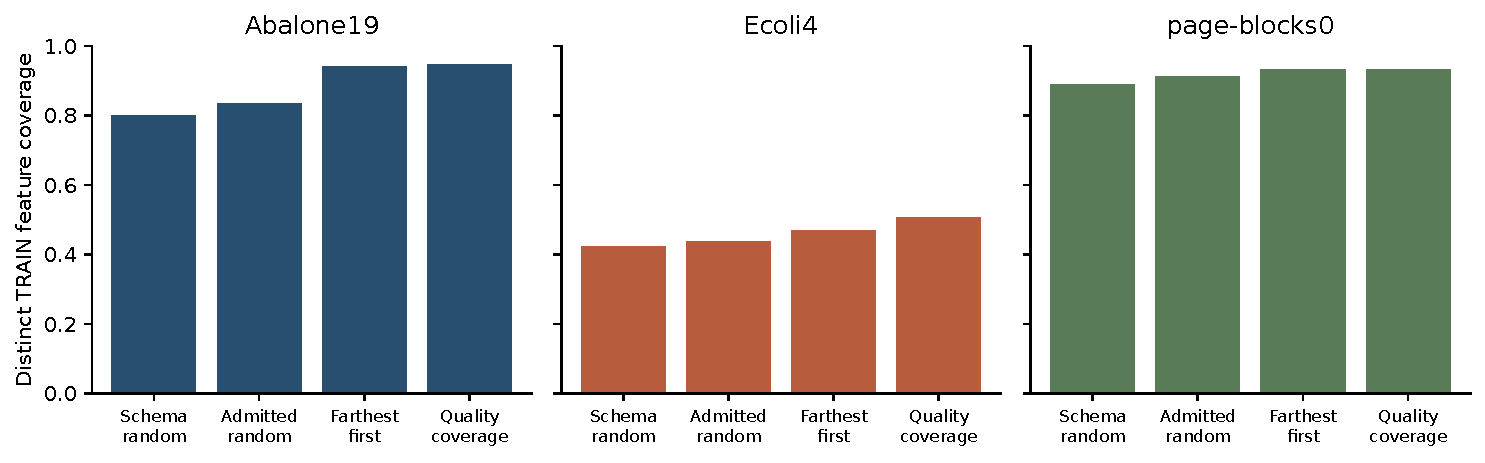
\includegraphics[width=\linewidth]{figures/coverage.pdf}
\caption{Historical fixed-budget distinct-feature TRAIN coverage. Random bars average five selection seeds; admitted selectors share the same pool.}\label{fig:coverage}\end{figure}

\subsection{RQ4: bounded repair}
All 54 eligible repairs become structurally compliant; 21 rejected records are ineligible. Repairs edit 73 fields: 39 records require one edit, eleven two and four three. Absolute changes range $.1$--$.5$, mean $.3119$. Five fractional-integer records also lack class and five require over three edits; neither group is repaired. Eleven further ineligible records belong to Abalone19/Ecoli4.

Under unchanged admission, 49 derived versions provisionally pass and five require review. The page-blocks0 admitted pool grows 119 to 168. At budget 49, quality-coverage selects 16 derived records: distinct-feature coverage rises $.9324$ to $.9370$, near duplication falls $.3265$ to $.1020$ and exact duplication remains zero. Source-order coverage slightly declines; other datasets are unchanged. Expanded pools therefore have method-dependent effects.

\subsection{RQ5: utility and external comparators}
All 138 historical utility rows reproduce within $10^{-12}$, including 24 unavailable cases. The expanded study contains 894 utility rows: 678 successful and 216 explicitly unavailable, without execution failures or budget shortfalls. Complete files retain both classifiers, regimes, class counts, confusion counts and metrics. Eighteen additional method/type incompatibilities are listed separately.

\begingroup\small\begin{longtable}{lrrrrrr}
\caption{Historical external training baselines. ROS and SMOTE/NC append b minority rows. LR: logistic regression; RF: random forest. These differ from candidate curation.}\label{tab:external}\\
\toprule
Dataset / method & Model & $+n$ & F1 & AP & BA & MCC \\
\midrule\endfirsthead
\toprule
Dataset / method & Model & $+n$ & F1 & AP & BA & MCC \\
\midrule\endhead
Abalone19 / Real & LR & 0 & 0.000 & 0.026 & 0.500 & 0.000 \\
Abalone19 / Real & RF & 0 & 0.000 & 0.023 & 0.500 & 0.000 \\
Abalone19 / Weighted LR & LR & 0 & 0.054 & 0.038 & 0.873 & 0.144 \\
Abalone19 / ROS+b & LR & 56 & 0.000 & 0.031 & 0.500 & 0.000 \\
Abalone19 / ROS+b & RF & 56 & 0.000 & 0.031 & 0.500 & 0.000 \\
Abalone19 / SMOTENC+b & LR & 56 & 0.000 & 0.014 & 0.499 & -0.003 \\
Abalone19 / SMOTENC+b & RF & 56 & 0.000 & 0.020 & 0.499 & -0.003 \\
Ecoli4 / Real & LR & 0 & 1.000 & 1.000 & 1.000 & 1.000 \\
Ecoli4 / Real & RF & 0 & 0.667 & 1.000 & 0.750 & 0.696 \\
Ecoli4 / Weighted LR & LR & 0 & 0.800 & 1.000 & 0.984 & 0.803 \\
Ecoli4 / ROS+b & LR & 70 & 1.000 & 1.000 & 1.000 & 1.000 \\
Ecoli4 / ROS+b & RF & 70 & 0.857 & 1.000 & 0.875 & 0.859 \\
Ecoli4 / SMOTE+b & LR & 70 & 1.000 & 1.000 & 1.000 & 1.000 \\
Ecoli4 / SMOTE+b & RF & 70 & 0.857 & 1.000 & 0.875 & 0.859 \\
page-blocks0 / Real & LR & 0 & 0.715 & 0.746 & 0.802 & 0.699 \\
page-blocks0 / Real & RF & 0 & 0.869 & 0.921 & 0.911 & 0.856 \\
page-blocks0 / Weighted LR & LR & 0 & 0.721 & 0.768 & 0.903 & 0.696 \\
page-blocks0 / ROS+b & LR & 49 & 0.728 & 0.746 & 0.811 & 0.712 \\
page-blocks0 / ROS+b & RF & 49 & 0.864 & 0.920 & 0.906 & 0.851 \\
page-blocks0 / SMOTE+b & LR & 49 & 0.728 & 0.758 & 0.811 & 0.712 \\
page-blocks0 / SMOTE+b & RF & 49 & 0.869 & 0.916 & 0.911 & 0.856 \\
\bottomrule\end{longtable}
\endgroup
External training baselines retain actual training populations and generated structural-compliance counts. Standard SMOTE's page-blocks0 outputs are not integer-coerced. Class weighting changes the training objective without generating records. These interventions are not matched candidate-curation alternatives.
In the historical page-blocks0 SMOTE baseline, 46 of 49 generated rows fail the integer structural contract; all remain computationally evaluable numerical augmentation records, and this incompatibility is explicit rather than repaired silently.

For historical page-blocks0 logistic pure TSTR, repair-pool expansion changes F1 from $.4464$ to $.3421$, while AP changes $.5552$ to $.5716$. Hybrid F1 stays $.7150$. This negative result accompanies improved coverage and near redundancy: geometric gains do not ensure utility gains.

\subsection{RQ6: conditional uncertainty and fresh-split stability}
\begingroup\scriptsize\setlength{\tabcolsep}{2pt}\begin{longtable}{lrrrrr}
\caption{Conditional 95\% bootstrap intervals (2,000 stratified paired resamples). Q: quality-coverage pure TSTR; Real: TRTR. Degenerate MCC intervals are unavailable; all valid counts are saved.}\label{tab:bootstrap}\\
\toprule
Dataset / method & Model & F1 [CI] & AP [CI] & BA [CI] & MCC [CI] \\
\midrule\endfirsthead
\toprule
Dataset / method & Model & F1 [CI] & AP [CI] & BA [CI] & MCC [CI] \\
\midrule\endhead
Abalone19 / Real & LR & 0.000 [0.000, 0.000] & 0.026 [0.022, 0.044] & 0.500 [0.500, 0.500] & 0.000 [--, --] \\
Abalone19 / Real & RF & 0.000 [0.000, 0.000] & 0.023 [0.012, 0.047] & 0.500 [0.500, 0.500] & 0.000 [--, --] \\
Abalone19 / Q & LR & 0.031 [0.029, 0.034] & 0.019 [0.012, 0.068] & 0.775 [0.758, 0.791] & 0.093 [0.087, 0.100] \\
Abalone19 / Q & RF & 0.030 [0.018, 0.039] & 0.021 [0.011, 0.046] & 0.724 [0.553, 0.820] & 0.078 [0.018, 0.112] \\
Abalone19 / Q repair & LR & 0.031 [0.029, 0.034] & 0.019 [0.012, 0.068] & 0.775 [0.758, 0.791] & 0.093 [0.087, 0.100] \\
Abalone19 / Q repair & RF & 0.030 [0.018, 0.039] & 0.021 [0.011, 0.046] & 0.724 [0.553, 0.820] & 0.078 [0.018, 0.112] \\
Ecoli4 / Real & LR & 1.000 [1.000, 1.000] & 1.000 [1.000, 1.000] & 1.000 [1.000, 1.000] & 1.000 [1.000, 1.000] \\
Ecoli4 / Real & RF & 0.667 [0.000, 1.000] & 1.000 [1.000, 1.000] & 0.750 [0.500, 1.000] & 0.696 [0.489, 1.000] \\
Ecoli4 / Q & LR & 0.205 [0.170, 0.258] & 0.135 [0.109, 0.267] & 0.754 [0.690, 0.817] & 0.241 [0.188, 0.307] \\
Ecoli4 / Q & RF & 0.296 [0.235, 0.400] & 0.633 [0.348, 1.000] & 0.849 [0.794, 0.905] & 0.349 [0.280, 0.450] \\
Ecoli4 / Q repair & LR & 0.205 [0.170, 0.258] & 0.135 [0.109, 0.267] & 0.754 [0.690, 0.817] & 0.241 [0.188, 0.307] \\
Ecoli4 / Q repair & RF & 0.296 [0.235, 0.400] & 0.633 [0.348, 1.000] & 0.849 [0.794, 0.905] & 0.349 [0.280, 0.450] \\
page-blocks0 / Real & LR & 0.715 [0.637, 0.783] & 0.746 [0.663, 0.832] & 0.802 [0.754, 0.845] & 0.699 [0.619, 0.769] \\
page-blocks0 / Real & RF & 0.869 [0.819, 0.914] & 0.921 [0.868, 0.965] & 0.911 [0.872, 0.944] & 0.856 [0.802, 0.904] \\
page-blocks0 / Q & LR & 0.446 [0.395, 0.500] & 0.555 [0.458, 0.656] & 0.759 [0.715, 0.804] & 0.389 [0.325, 0.456] \\
page-blocks0 / Q & RF & 0.342 [0.308, 0.377] & 0.447 [0.368, 0.534] & 0.727 [0.685, 0.768] & 0.288 [0.234, 0.342] \\
page-blocks0 / Q repair & LR & 0.342 [0.303, 0.383] & 0.572 [0.482, 0.676] & 0.713 [0.669, 0.758] & 0.278 [0.222, 0.337] \\
page-blocks0 / Q repair & RF & 0.316 [0.283, 0.350] & 0.474 [0.391, 0.572] & 0.704 [0.661, 0.748] & 0.254 [0.200, 0.309] \\
\bottomrule\end{longtable}
\endgroup
The 216 endpoint and 168 paired-difference intervals derive from saved predictions. Page-blocks0 logistic repair-minus-original F1 is approximately $-.1043$, with conditional interval $[-.1350,-.0739]$; AP difference is $.0165$, interval $[-.0071,.0493]$. F1 decreases consistently under this conditional resampling design, while AP direction is less stable. These remain descriptive intervals on reused historical TEST.

Ecoli4 logistic TRTR predicts perfectly on only four positive and 63 negative TEST records, yielding conditional F1 interval $[1,1]$. Its Wilson positive-recall interval is approximately $[.510,1]$. Resampling perfect observed predictions cannot establish universal performance. Abalone19 has only six positive TEST examples; resampling adds no independent positive observations.

\begingroup\scriptsize\begin{longtable}{lrrrrr}
\caption{Offline replication: five repeated stratified holdouts, logistic regression, mean $\pm$ sample SD. Real and weighted are TRTR; other methods are hybrid minority augmentation. No historical candidates are reused.}\label{tab:repeated}\\
\toprule
Dataset / method & $k$ & F1 & AP & BA & MCC \\
\midrule\endfirsthead
\toprule
Dataset / method & $k$ & F1 & AP & BA & MCC \\
\midrule\endhead
Abalone19 / Weighted LR & 5 & 0.051 $\pm$ 0.009 & 0.045 $\pm$ 0.014 & 0.779 $\pm$ 0.071 & 0.116 $\pm$ 0.028 \\
Abalone19 / Real & 5 & 0.000 $\pm$ 0.000 & 0.042 $\pm$ 0.015 & 0.500 $\pm$ 0.000 & 0.000 $\pm$ 0.000 \\
Abalone19 / ROS+b & 5 & 0.000 $\pm$ 0.000 & 0.040 $\pm$ 0.014 & 0.500 $\pm$ 0.001 & -0.002 $\pm$ 0.002 \\
Abalone19 / SMOTENC+b & 5 & 0.000 $\pm$ 0.000 & 0.041 $\pm$ 0.013 & 0.500 $\pm$ 0.000 & -0.002 $\pm$ 0.002 \\
Abalone19 / Curated Q & 5 & 0.000 $\pm$ 0.000 & 0.044 $\pm$ 0.011 & 0.500 $\pm$ 0.001 & -0.002 $\pm$ 0.002 \\
Abalone19 / Admitted random & 5 & 0.000 $\pm$ 0.000 & 0.047 $\pm$ 0.016 & 0.500 $\pm$ 0.000 & -0.001 $\pm$ 0.002 \\
Abalone19 / Schema random & 5 & 0.000 $\pm$ 0.000 & 0.041 $\pm$ 0.012 & 0.500 $\pm$ 0.000 & -0.002 $\pm$ 0.002 \\
Ecoli4 / Weighted LR & 5 & 0.695 $\pm$ 0.117 & 0.923 $\pm$ 0.053 & 0.928 $\pm$ 0.074 & 0.692 $\pm$ 0.127 \\
Ecoli4 / Real & 5 & 0.848 $\pm$ 0.119 & 0.944 $\pm$ 0.058 & 0.875 $\pm$ 0.088 & 0.855 $\pm$ 0.108 \\
Ecoli4 / ROS+b & 5 & 0.745 $\pm$ 0.177 & 0.908 $\pm$ 0.055 & 0.865 $\pm$ 0.089 & 0.744 $\pm$ 0.182 \\
Ecoli4 / SMOTE+b & 5 & 0.758 $\pm$ 0.166 & 0.944 $\pm$ 0.058 & 0.867 $\pm$ 0.089 & 0.757 $\pm$ 0.170 \\
Ecoli4 / Curated Q & 5 & 0.758 $\pm$ 0.166 & 0.934 $\pm$ 0.050 & 0.867 $\pm$ 0.089 & 0.757 $\pm$ 0.170 \\
Ecoli4 / Admitted random & 5 & 0.758 $\pm$ 0.166 & 0.934 $\pm$ 0.050 & 0.867 $\pm$ 0.089 & 0.757 $\pm$ 0.170 \\
Ecoli4 / Schema random & 5 & 0.758 $\pm$ 0.166 & 0.944 $\pm$ 0.058 & 0.867 $\pm$ 0.089 & 0.757 $\pm$ 0.170 \\
page-blocks0 / Weighted LR & 5 & 0.708 $\pm$ 0.029 & 0.788 $\pm$ 0.024 & 0.913 $\pm$ 0.013 & 0.687 $\pm$ 0.031 \\
page-blocks0 / Real & 5 & 0.728 $\pm$ 0.026 & 0.800 $\pm$ 0.019 & 0.819 $\pm$ 0.025 & 0.709 $\pm$ 0.025 \\
page-blocks0 / ROS+b & 5 & 0.738 $\pm$ 0.028 & 0.800 $\pm$ 0.019 & 0.828 $\pm$ 0.028 & 0.718 $\pm$ 0.029 \\
page-blocks0 / SMOTE+b & 5 & 0.736 $\pm$ 0.033 & 0.800 $\pm$ 0.019 & 0.826 $\pm$ 0.031 & 0.715 $\pm$ 0.032 \\
page-blocks0 / Curated Q & 5 & 0.738 $\pm$ 0.028 & 0.800 $\pm$ 0.020 & 0.828 $\pm$ 0.029 & 0.718 $\pm$ 0.029 \\
page-blocks0 / Admitted random & 5 & 0.741 $\pm$ 0.027 & 0.799 $\pm$ 0.019 & 0.829 $\pm$ 0.030 & 0.721 $\pm$ 0.026 \\
page-blocks0 / Schema random & 5 & 0.736 $\pm$ 0.030 & 0.800 $\pm$ 0.019 & 0.826 $\pm$ 0.029 & 0.716 $\pm$ 0.029 \\
\bottomrule\end{longtable}
\endgroup
All 15 split-specific runs complete. Ecoli4 logistic F1 is $.8476\pm.1186$ for real-only training and $.7581\pm.1659$ for quality-curated augmentation. Admitted random has the same mean F1 there, though ranking metrics differ. Abalone19 logistic F1 stays zero under real-only and the declared augmentation methods; balanced logistic loss reaches $.0506\pm.0095$. On page-blocks0, real-only F1 is $.7284\pm.0256$, quality-curated augmentation $.7383\pm.0283$ and admitted random $.7409\pm.0270$. These outcomes do not show a uniform augmentation benefit or superiority over simple curation.

\begin{figure}[htbp]\centering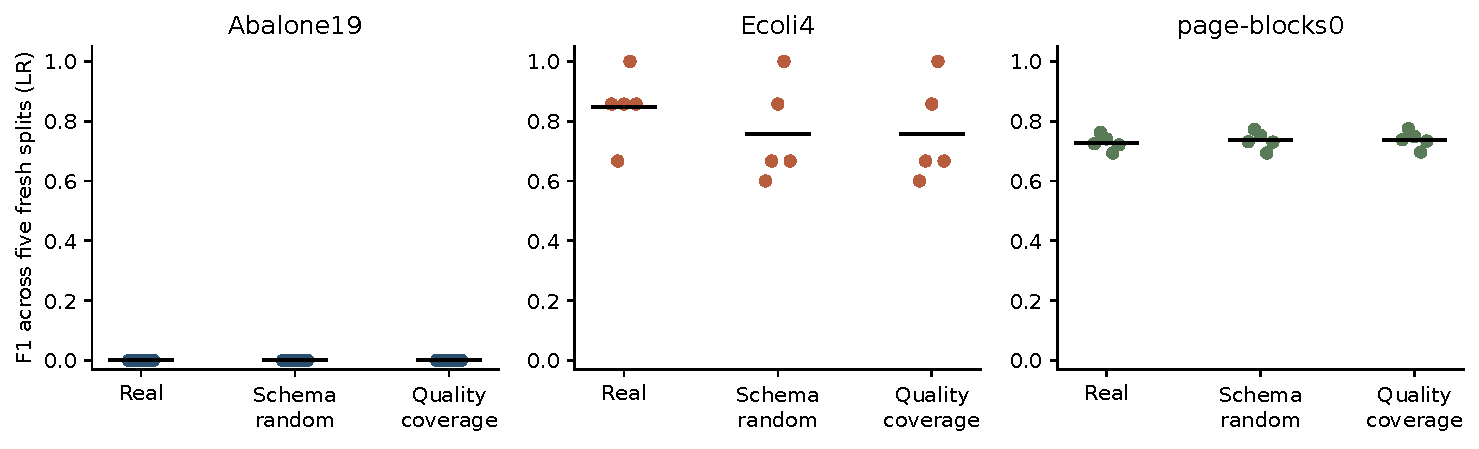
\includegraphics[width=\linewidth]{figures/repeated-f1.pdf}
\caption{Every fresh-split logistic F1 value; black bars show five-split means. Real-only and hybrid regimes are distinct. The page-blocks0 pool generator is ROS.}\label{fig:repeated}\end{figure}
Split-wise paired differences use identical evaluation records. Pure TSTR on offline minority-only pools is unavailable, never renamed hybrid augmentation.

\section{Discussion}
The strongest empirical contribution is a measurable separation of compliance, support, geometry and utility. Structural defects occur often enough in this historical stream to motivate explicit checks, and narrow repair corrects an eligible subset without fabricating labels. Coverage-oriented construction can reduce redundancy, but its classifier consequences remain mixed. Geometric evidence should therefore accompany direct task evaluation.

Admission ablations estimate the effect of changing candidate availability under fixed downstream rules, not a score's isolated utility effect with selected identities held constant. Repair changes both pool and selection; its utility decrease cannot be assigned solely to rounding one field. Source order can exclude the minority entirely, making unavailable TSTR a meaningful result rather than justification for adding ineligible data.

Simple alternatives are informative. Farthest-first eliminates duplicates, random selection remains competitive offline, and balanced logistic loss gives nonzero Abalone19 F1 where fixed-budget augmentation does not. The contribution is auditable curation with explicit tradeoffs rather than universally superior classifier training.

\section{Limitations}
The historical study uses three datasets, a previously evaluated TEST and recorded exact-feature TRAIN/TEST overlap. Full original TRAIN influenced generation, preventing independent split claims from that pool. The fresh study rebuilds all fitted objects and candidates, but holdouts overlap and generators differ from the LLM stream. ROS adds no new support, and minority-only pools preclude pure TSTR. Offline findings do not establish LLM-generation replication.

Four and six historical TEST positives limit Ecoli4 and Abalone19 inference. Stratified intervals condition on observed records and fixed models; they do not quantify generation/refitting uncertainty or discover unseen positive modes. Undefined MCC margins are excluded with counts reported, potentially changing the conditional target. Comparisons are exploratory, without multiplicity-adjusted significance or state-of-the-art claims.

Source declarations establish a limited contract. Physical constraints, original target meaning and cross-field semantics remain unresolved where sources cannot justify them. No human annotation experiment is conducted, so complete semantic validity is not independently established. Evidence remains uncalibrated and provisional admission is a selection policy, not verified validity. Distances depend on scaling, support and covariance assumptions; coverage establishes neither predictive accuracy nor privacy.

\section{Conclusion}
RC-QASyn makes provenance, structural compliance, statistical support, fixed-budget construction and bounded repair inspectable within the existing six-phase system. The historical audit identifies 75 structural rejects, corrects all 54 eligible records and measures changes in coverage and redundancy. Paired uncertainty and fresh train-only offline experiments strengthen the evidence while revealing limited and sometimes negative utility effects. The contribution is an empirically bounded, reproducible account of curation tradeoffs.

\section*{Declarations}
\textbf{Authors/affiliations/CRediT:} Human authors must supply accurate names, institutions, roles and contact information before submission.

\textbf{Funding, conflicts and ethics:} Human authors must complete institutional and venue declarations; no approval, exemption or absence of conflicts/funding is inferred. Human validity annotation is outside this study.

\textbf{Data/code:} Versioned local source, manifests, generated-pool provenance, paired predictions, metrics, unavailable reasons and editable manuscript accompany this revision. Public release and licensing require author review. No remote push or merge is implied.

\textbf{AI assistance:} An AI coding/drafting assistant supported implementation, orchestration, source checking and revision under researcher instructions. Human authors must verify the work, accept submission responsibility and adapt this declaration to institutional/venue requirements. AI is not an author.

\bibliographystyle{plainnat}
\bibliography{references}
\appendix
\section{Class denominators and confusion counts}
\begingroup\small\begin{longtable}{lrrrrrrr}
\caption{Historical primary predictions: class denominators and confusion counts. Q and Q repair use pure TSTR; Real uses TRTR.}\label{tab:confusions}\\
\toprule
Dataset / method & Model & $n_+$ & $n_-$ & TP & FP & TN & FN \\
\midrule\endfirsthead
\toprule
Dataset / method & Model & $n_+$ & $n_-$ & TP & FP & TN & FN \\
\midrule\endhead
Abalone19 / Real & LR & 6 & 828 & 0 & 0 & 828 & 6 \\
Abalone19 / Real & RF & 6 & 828 & 0 & 0 & 828 & 6 \\
Abalone19 / Q & LR & 6 & 828 & 6 & 373 & 455 & 0 \\
Abalone19 / Q & RF & 6 & 828 & 5 & 319 & 509 & 1 \\
Abalone19 / Q repair & LR & 6 & 828 & 6 & 373 & 455 & 0 \\
Abalone19 / Q repair & RF & 6 & 828 & 5 & 319 & 509 & 1 \\
Ecoli4 / Real & LR & 4 & 63 & 4 & 0 & 63 & 0 \\
Ecoli4 / Real & RF & 4 & 63 & 2 & 0 & 63 & 2 \\
Ecoli4 / Q & LR & 4 & 63 & 4 & 31 & 32 & 0 \\
Ecoli4 / Q & RF & 4 & 63 & 4 & 19 & 44 & 0 \\
Ecoli4 / Q repair & LR & 4 & 63 & 4 & 31 & 32 & 0 \\
Ecoli4 / Q repair & RF & 4 & 63 & 4 & 19 & 44 & 0 \\
page-blocks0 / Real & LR & 112 & 983 & 69 & 12 & 971 & 43 \\
page-blocks0 / Real & RF & 112 & 983 & 93 & 9 & 974 & 19 \\
page-blocks0 / Q & LR & 112 & 983 & 75 & 149 & 834 & 37 \\
page-blocks0 / Q & RF & 112 & 983 & 85 & 300 & 683 & 27 \\
page-blocks0 / Q repair & LR & 112 & 983 & 78 & 266 & 717 & 34 \\
page-blocks0 / Q repair & RF & 112 & 983 & 84 & 336 & 647 & 28 \\
\bottomrule\end{longtable}
\endgroup
\section{Paired repair intervals}
\begingroup\small\begin{longtable}{lrrrrr}
\caption{Repair-pool minus original Q, logistic pure TSTR: conditional paired difference intervals. These measure pool expansion and reselection together.}\label{tab:paired}\\
\toprule
Dataset & Metric & Lower & Upper & Valid & Undefined \\
\midrule\endfirsthead
\toprule
Dataset & Metric & Lower & Upper & Valid & Undefined \\
\midrule\endhead
Abalone19 & f1 & 0.000 & 0.000 & 2000 & 0 \\
Abalone19 & average\_precision & 0.000 & 0.000 & 2000 & 0 \\
Abalone19 & balanced\_accuracy & 0.000 & 0.000 & 2000 & 0 \\
Abalone19 & mcc & 0.000 & 0.000 & 2000 & 0 \\
Ecoli4 & f1 & 0.000 & 0.000 & 2000 & 0 \\
Ecoli4 & average\_precision & 0.000 & 0.000 & 2000 & 0 \\
Ecoli4 & balanced\_accuracy & 0.000 & 0.000 & 2000 & 0 \\
Ecoli4 & mcc & 0.000 & 0.000 & 2000 & 0 \\
page-blocks0 & f1 & -0.135 & -0.074 & 2000 & 0 \\
page-blocks0 & average\_precision & -0.007 & 0.049 & 2000 & 0 \\
page-blocks0 & balanced\_accuracy & -0.067 & -0.024 & 2000 & 0 \\
page-blocks0 & mcc & -0.146 & -0.075 & 2000 & 0 \\
\bottomrule\end{longtable}
\endgroup
All primary pairs for both classifiers and available regimes are in \texttt{paired-differences.json}. Undefined counts remain per endpoint. \texttt{confusions.csv} retains confusion counts and Wilson recall bounds for every successful result.

\section{Evidence map and reproduction}
The protocol is \path{docs/empirical-v2/protocol.md}; machine settings are in \path{configs/empirical/protocol-v1.json}. Canonical evidence is \path{artifacts/reports/empirical-v2/run-v2}. The report includes consolidated ablations, split-wise paired differences and confusions. A development run is explicitly superseded for an interval-metadata naming defect; its scores never selected configurations.

With this revision's \texttt{src} on PYTHONPATH, run \texttt{scripts/run\_empirical\_study.py} using a fresh output directory and frozen checkout as \texttt{--source-root}. \texttt{scripts/report\_empirical\_study.py} reads saved evidence without refitting. Exact commands, pinned dependencies and verification are in \texttt{docs/empirical-v2/handoff.md}.

The manifest binds revisions, code hashes, protocol identity, dependencies, runtime and output hashes. Population records retain exact TRAIN/TEST identities, source/dataset fingerprints, class counts and overlap diagnostics. Generator files retain fitted TRAIN identities, scaler parameters, seeds and generated payloads. Existing M2/M7 use fresh split-specific populations. Predictions preserve actual/predicted classes, positive scores and row identity; compressed index arrays preserve paired resamples.

The cell ledger \texttt{notes/table-evidence.json} links rendered values to input fields, row fingerprints and aggregation rules. Original M2, M4 and M6/M7 sensitivities remain unchanged. Individual seeds, every split, both classifiers, unavailable cases and budget checks accompany the paper. Full regression/static checks, replay and historical integrity are reported separately; replay is not another independent split.

\end{document}
